\section{Individual Mirror Control}
\label{sec:mirror}

The pan and tilt of each mirror unit is driven by a pair of
unipolar 12V stepper motors, commanded over an I2C bus by an
Arduino Uno\footnote{\url{https://www.arduino.cc}} on either end of
each row of mirrors (see Figure~\ref{fig:mirror})~\cite{acadia18}.
The two halves (east and west) have a
Raspberry~Pi\footnote{\url{https://www.raspberrypi.org}}
communicating with the Arduino Unos over USB, which also provides
wireless connectivity to a remote PC running Rhino3D/Grasshopper.

\begin{figure}[ht]
\centering
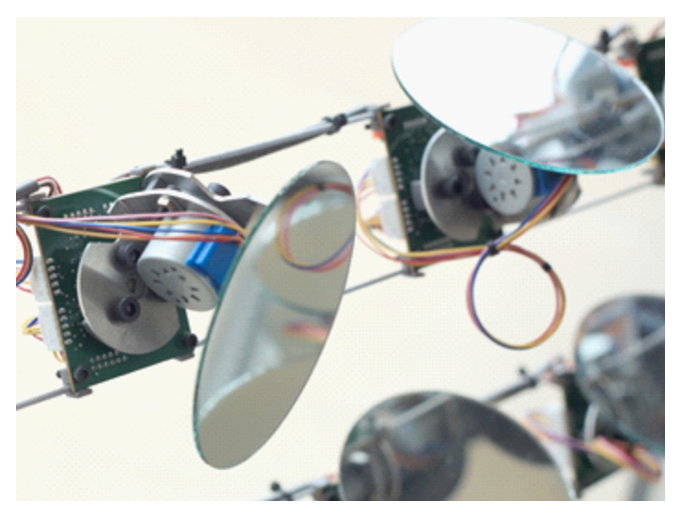
\includegraphics[width=0.98\columnwidth]{mirror}
\caption{Individual mirror units,
each with pan and tilt control~\protect\cite{acadia18}.}
\label{fig:mirror}
\end{figure}

The stepper motors are running open loop,
(i.e., there are no shaft encoders in the system),
so to establish known position each
motor is driven to the physical stops (a reset position) and then
the Arduino Unos accept motor movement commands that include
mirror ID ($x$ and $y$ position in the surface), which motor (pan vs.\ tilt),
direction, and number of steps.
The local Arduino Unos make no
attempt to retain position information, as that is the responsibility
of the higher-level system.

To enable movement profiles, we will extend the messaging protocol
and use the Arduino Unos to provide more nuanced timing in their
motor movement commands. This is fairly straightforward in a stepper
motor-driven system, in which individual step control is available.

The resulting catoptric surface is effectively an IoT device, which
relies on network connectivity for high-level control.
